%% This is based on the leaflet.tex file present in the texlive-leaflet module
%% 
%% Copyright 2014 Ankur Sinha for the Fedora Marketing Team - marketing@lists.fedoraproject.org
% Please e-mail the marketing team if you have any questions with this document

\def\filename{fedora-flyer-workstation.tex}
\documentclass[
%%notumble,
%%nofoldmark,
%%dvipdfm,
%%portrait,
%%titlepage,
%%nocombine,
%%a3paper,
%%debug,
%%nospecialtricks,
%%draft,
letterpaper,
10pt
]{leaflet}


%\renewcommand*\foldmarkrule{.3mm}
%\renewcommand*\foldmarklength{5mm}

\usepackage[T1]{fontenc}
\usepackage{textcomp}
% Use this to change the paper format
\usepackage{fancyhdr}
\usepackage{graphicx}
\usepackage[none]{hyphenat}

%%\usepackage[default]{cantarell} %% Use option ``defaultsans'' to use cantarell as sans serif only
%%\usepackage[default]{comfortaa} %% looks better
%%\usepackage[T1]{fontenc}

%% helvetica
%\usepackage{helvet}
%\renewcommand*{\familydefault}{\sfdefault}
% opensans
\usepackage[default,osfigures,scale=0.95]{opensans} %% Alternatively

\usepackage[dvipsnames,usenames]{color}
\definecolor{FedoraBlue}{cmyk}{1,0.46,0,0}
\definecolor{ResolutionBlue}{cmyk}{0.573,.462,0,0.541}
\definecolor{LIGHTGRAY}{gray}{.9}
\usepackage[colorlinks=true,urlcolor=FedoraBlue]{hyperref}

%%\setlength\footskip{2cm}

\newcommand*\defaultmarker{\textsuperscript\textasteriskcentered}

%%\title{Fedora workstation}
\title{
\includegraphics[keepaspectratio,width=0.8\textwidth]{Logo_fedoralogo.png}\vspace{1cm}\\
\includegraphics[keepaspectratio,scale=0.5]{workstation_logo_only.png}\\\vspace{0.5cm}\LARGE{\textcolor{ResolutionBlue}{WORKSTATION}}}
\author{\LARGE{\textcolor{ResolutionBlue}{22}}}
\date{\href{http://ask.fedoraproject.org}{http://ask.fedoraproject.org}}

\CutLine*{1}% Dotted line without scissors
%%\CutLine{6}%  Dotted line with scissors
\CutLine*{6}%  Dotted line with scissors

%% Use better logo for the workstation
%%\AddToBackground{1}{%  Background of a small page
%%  \put(20,530){
\includegraphics{workstation-logo.png}}}

%\AddToBackground{5}{%  Background of a small page
%  \put(0,0){\textcolor{Cerulean}{\rule{\paperwidth}{\paperheight}}}}
%%
\AddToBackground*{2}{% Background of a large page
  \put(\LenToUnit{.5\paperwidth},\LenToUnit{.5\paperheight}){%
    \makebox(0,0)[c]{%
      \resizebox{.9\paperwidth}{!}{\rotatebox{35.26}{%
        \textsf{\textbf{\textcolor{LIGHTGRAY}{DRAFT}}}}}}}}

\begin{document}

\maketitle
\thispagestyle{empty}
\vspace{5cm}
\begin{center}\small{Fedora and the Infinity Logo are\\registered trademarks of Red Hat, Inc.}\end{center}

\newpage


\section{\textcolor{FedoraBlue}{Easy access to all your software}}
\begin{figure}[h]
  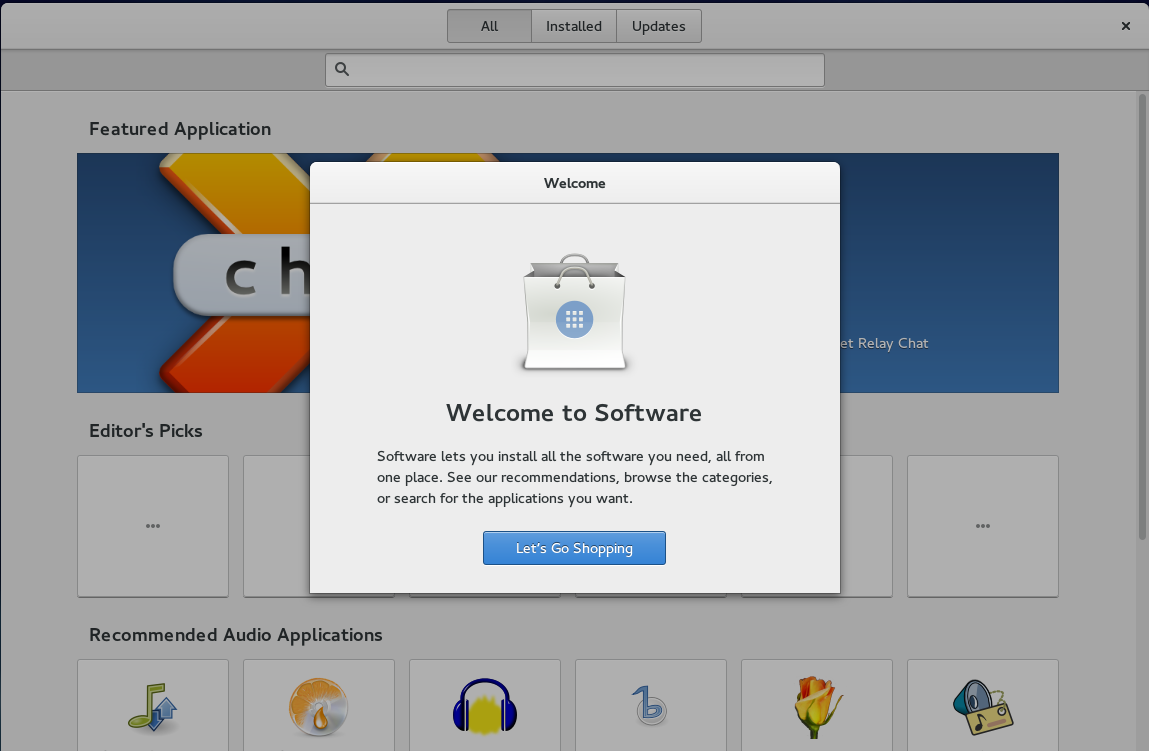
\includegraphics[keepaspectratio,width=\textwidth]{Gnome_software_welcome-cropped.png}
\end{figure}
The cornerstone of the Fedora Workstation is the Software installer, which lets you find all kinds of applications quickly and easily. The application now has more and better data than ever before, and makes it easy for you to find a variety of useful free software. It also helps you install extras such as fonts and media helpers, and even lets you easily update your Fedora workstation!

\section{\textcolor{FedoraBlue}{Refined themes}}
The GNOME Shell and other themes and design are refined and improved. Now you can more easily identify information on the screen, adjust window size and placement, and navigate your files and folders. Improved bridging between desktop environment themes allows applications from other environments like KDE to look and feel more like native applications as they're updated to take advantage of this feature. Standard scrollbars have been replaced by a minimal, overlaid indicator, while a scrollbar trough is shown when needed. This create a cleaner, less distracting view which helps you focus on window content. These ``overlay scrollbars'' are also better suited to mouse scroll wheels and touch pad scrolling.

\section{\textcolor{FedoraBlue}{Better notifications}}
\begin{figure}[h]
  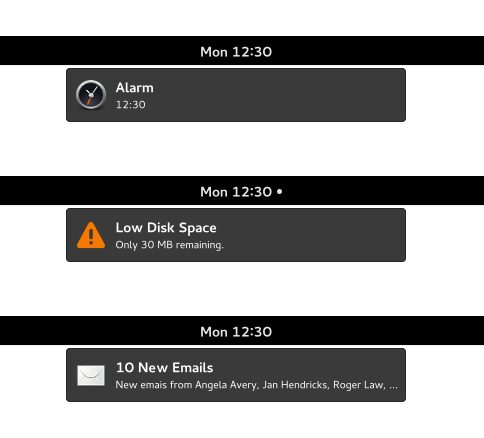
\includegraphics[keepaspectratio,width=\textwidth]{notifications-f22-cropped.png}
\end{figure}
Thanks both to work done in GNOME 3.16 and other projects like the Automatic Bug Reporting Tool (ABRT), notifications keep you better informed, but interfere less with your work. They now appear anchored to the center of the top bar, and no longer cover up the bottom of the screen where you are often reading a terminal or browser. An unobtrusive marker appears in the calendar to let you know you have unread notifications. If ABRT detects a serious bug, a friendly notification appears and allows you to report the bug information, but doesn't overload you with details. And if you're a serious Terminal user, longer background jobs now notify you when they're done, so you can get on with other work and pick up the results when you're ready. 

\section{\textcolor{FedoraBlue}{Nautilus improvements}}
\begin{figure}[h]
  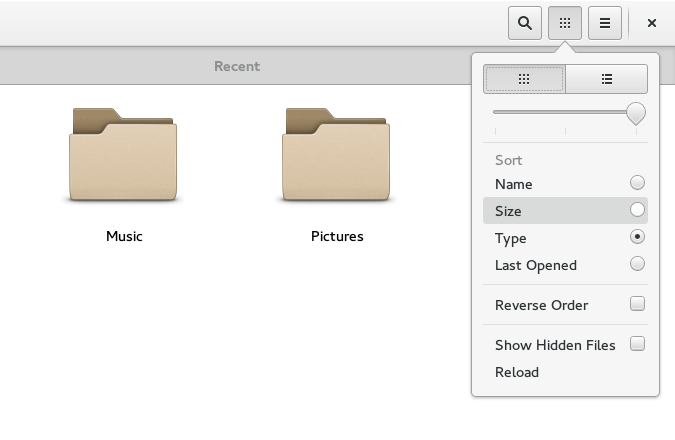
\includegraphics[keepaspectratio,width=\textwidth]{nautilus-f22-cropped.png}
\end{figure}
The updated layout in Files gives a better view of your files and folders, and a new view popover makes it easy to change the zoom level and sort order from a single place. You can also now move files and folders to the trash intuitively using the Delete key, rather than the Ctrl+Delete keyboard combination. 

\section{\textcolor{FedoraBlue}{Other improvements}}
Of course, that's not all. Other applications have seen improvements too:
\begin{itemize}
  \item The user interface for \textbf{Boxes}, the application for virtual and remote machines, has a large number of improvements, including new preferences dialogs, a revamped box creation assistant, a feature to send keyboard shortcuts to a box, and display scaling by default.
  \item Developers will appreciate the addition of software development environment software \textbf{Vagrant} into Fedora -- it'll work using our included virtualization technology, with no need to install third-party virtualization (like VirtualBox). Use this to work on top of the Cloud images mentioned above, or launch your own Vagrant boxes.
  \item The \textbf{Image Viewer} has been redesigned to reduce the amount of window chrome and give more space to images. 
  \item Faster and better dependency management with \textbf{DNF}.
  \item \textbf{Elasticsearch} is full-featured and very popular self-standing open source indexing server, and now it's available by with just a ``yum install elasticsearch'' -- no, wait, make that ``dnf install elasticsearch''! 
  \item Fedora 22 comes with \textbf{GNU Compiler Collection 5.1} as the primary compiler suite.
  \item \ldots and much more
\end{itemize}

\section{\textcolor{FedoraBlue}{Exciting roadmap}}
The community continues to work towards making Fedora a better \href{http://www.gnu.org/philosophy/free-sw.en.html}{free} operating system for our users.  So if you want to be part of the future of the Linux desktop, get on board now!

Information on the complete roadmap can be found here:\\ \href{http://fedoraproject.org/wiki/Releases/22/ChangeSet}{http://fedoraproject.org/wiki/Releases/22/ChangeSet}

\vspace{1.5cm}
\begin{figure}[h]
  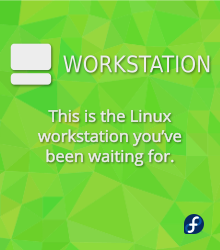
\includegraphics[keepaspectratio,width=\textwidth]{Fedora-workstation-v5a-infinity.png}
\end{figure}
\newpage

\begin{center}
  {\color{FedoraBlue}
  \LARGE{Fedora Project\vspace{1cm}}
  \Large{\href{http://fedoraproject.org}{http://fedoraproject.org}}
}
\end{center}

\section{\textcolor{FedoraBlue}{Getting Support}}
\subsection{Fedora project wiki and mailing lists}
\href{https://fedoraproject.org/wiki/Communicate}{https://fedoraproject.org/wiki/Communicate}

\subsection{Official Documentation}
\href{http://docs.fedoraproject.org}{http://docs.fedoraproject.org}

\subsection{IRC Channel}
\href{http://webchat.freenode.net/?channels=#fedora}{\#fedora @ irc.freenode.net}

\subsection{Community forums}
\href{http://ask.fedoraproject.org}{http://ask.fedoraproject.org}
\href{http://fedoraforum.org}{http://fedoraforum.org}


\section{\textcolor{FedoraBlue}{Looking to join the Fedora community?}}
Are you interested in contributing to Fedora? There are many ways you can become active in the project.  Whether you are a People Person, Designer, OS Developer, Packager or Administrator - we have a place for you. Just head to the following page and get started today!

\begin{center}\href{http://join.fedoraproject.org}{http://join.fedoraproject.org}\end{center}


\end{document}
